\section{Experimenteller Teil}
Im ersten Teil der Auswertung verfolgen wir im Wesentlichen Ionen durch die Anlage.
Untersucht werden soll dabei eine vorbereitete BeO-Probe.
Im zweiten Teil betrachten wir aufgenommene Spektren und untersuchen eine unbekannte Probe.

\subsection{Auf dem Weg zum Beschleuniger}
Nach der Produktion der negativen Ionen durch sputtern werden diese direkt mit insgesamt \SI{29}{\kilo\electronvolt} beschleunigt.
Sie durchlaufen dann eine elektrostatischen Analysierer und einen ersten Ablenkmagneten.
Das Ziel hier ist eine Ionenmasse vorzuselektieren.
Da wir BeO untersuchen sind mögliche gesuchte Ionen $^{9}\text{Be}^{16}\text{O}^{-}$ (stabiles Beryllium-Iosotop) und $^{10}\text{Be}^{16}\text{O}^{-}$ (radioaktives Beryllium-Iostop mit einer Halbwertszeit von \num{1.51e6} Jahren).
Zu beachten ist, dass Sauerstoff zwar zum Großteil aus $^{16}$O besteht, jedoch in geringen Mengen auch die stabilen Isotope $^{17}$O und $^{18}$O vorkommen können, was eine geiwsse Quelle für Unsicherheiten ist.
Wir kennen die kinetische Energie $E_{\text{kin}}$, den Ladungszustand $q_{\text{ion}}$, die Masse der Ionen $m_{\text{ion}}$ und den Krümmungsradius der weiterführenden Trajektorie $\rho$.
Daher kann man durch geeignete Wahl der Stärke des Magnetfeldes die Ionenmasse auswählen:
\begin{gather}
    B \rho = \frac{p_{\text{ion}}}{q_{\text{ion}}} = \frac{\sqrt{2m_{\text{ion}}E_{\text{kin}}}}{q_{\text{ion}}}
    \label{Auswertung_eq_Magnet}
\end{gather}
Ionen mit einer anderen Masse oder anderem Ladungszustand haben im Magneten eine anders gekrümmte Trajektorie und gelangen daher nicht durch die Eintrittsöffnung zum Beschleuniger.
(Tatsächlich lässt sich wie in Gleichung \ref{Auswertung_eq_Magnet} zu sehen nur nach $\frac{\sqrt{m_{\text{ion}}}}{q_{\text{ion}}}$ selektieren.
Ionen mit vierfacher Masse und doppelter Ladung würden also auch weiterkommen. Derart schwere Teilchen sind jedoch fast gar nicht in der Probe vorhanden.)
Nicht unterscheiden lässt sich jedoch zwischen Molekularen isobaren, so zum Beispiel zwischen $^{10}\text{Be}^{16}\text{O}^{-}$ und $^{9}\text{Be}^{17}\text{O}^{-}$ (wobei $^{17}\text{O}$ in der Natur sehr selten vorkommt) oder $^{10}\text{Be}^{16}\text{O}^{-}$ und $^{10}\text{B}^{16}\text{O}^{-}$ ($^{10}\text{B}$ entsteht beim Beta-Zerfall von $^{10}\text{Be}$).
Für $\rho$ war ein Wert von \SI{0.4}{\metre} gegeben.
Damit ergeben sich für einfach negativ geladene Ionen folgende benötigte Magnetfeldstärken:
\begin{table}[h]
  \centering
  \begin{tabular}{|c|c|}
    \hline
    Ion & Magnetfeldstärke \\
    \hline
    $^{9}\text{Be}^{16}\text{O}^{-}$ & \SI{-0.306}{\tesla} \\
    \hline
    $^{10}\text{Be}^{16}\text{O}^{-}$ & \SI{-0.313}{\tesla} \\
    \hline
  \end{tabular}
  \caption{Benötigte Magnetfeldstärken im ersten Ablenkmagneten für Ionen vor dem Beschleuniger}
  \label{Auswertung_tab_Ionenenergien_vor_Besch}
\end{table}
Um diese Magnetfelder anzulegen ist eine Kalibrierung des Magneten erforderlich, die jedoch in diesem Versuch nicht durchgeführt wurde.
Stattdessen haben wir die chemisch reine Probe 153BeO genutzt, um die Stromstärke zu bestimmen, welche der Magnetfeldstärke zur Selektion von BeO$^{-1}$ entspricht.
Diese kann dann als Vergleichswert dienen um aus den Verhältnissen der Magnetfeldstärken bzw. Stromstärken die Teilchen zu identifizeren.
Dieses Verhältnis folgt aus Formel \ref{Auswertung_eq_mMagnet} zu $\frac{B_1}{B_2} = \sqrt{\frac{m_1}{m_2}}$.
Vor dem Tandem ergibt sich die Energie der BeO$^{-1}$ Teilchen zu $E = q \cdot U_{ionsource}$.
Nach Formel \ref{Auswertung_eq_Magnet}, mit dem Radius des Magneten $\rho = 0,4$ m, ergibt sich für das zugehörige Magnetfeld $T = 0,306$ T.
Messungen am Magneten ergaben eine zugehörige Stromstärke von $I = 61,05$ A.
Die Masse eines unbekannten Teilchens ergibt sich damit zu:
\begin{equation}
    m_2 = m_1 \cdot \left( \frac{B_2}{B_1} \right)^2 = 25 \: \text{u} \cdot \frac{I}{61.05 \: \text{A}}
    \label{LE_masse}
\end{equation}
Hier müssen wir als prinzipielle Unsicherheit beachten, dass sich Teilchen mit mehrfach negativer Ladung als Teilchen niedrigerer Masse detektiert werden (siehe Formel \ref{Auswertung_eq_Magnet}).
Unsicherheiten der Beschleunigungsspannungen und des Spulenradius werden hier nicht betrachtet, da sie gegenüber der variablen Hysterese des Magneten kaum einen Einfluss auf die Unsicherheit der Ablenkung haben.
Diese wiederrum wäre ebenfalls am besten experimentell (z.B. mittels Hall-Sonde) zu bestimmen.

In Abb. \ref{lowenergy} sind jetzt die Messungen dargestellt.
Zur Identifikation betrachten wir als erstes die 153BeO Probe, die berechneten Massen sind in Tab, \Ref{153Be} zu sehen.
Die höhe der Peaks wird für die folgende Analyse nicht betrachtet.
\begin{table}[h]
\centering
\caption{Berechnung der Massen im Niedrigenergiebereich für Probe 153Be.}
\begin{tabular}{|c |c|}
\hline
I[A] & m[u] \\
\hline
49,03 & 16,1 \\
61,31 & 25,2 \\
64,88 & 28,2 \\
\hline
\end{tabular}
\label{153Be}
\end{table}
Die entsprechenden Massen sind hier eindeutig zuordbar, was bei einer reinen Probe auch zu erwarten war.
\begin{itemize}
\item $16$ u entsprechen der Masse von $^{16}$O$^{1-}$.
\item $25$ u entsprechen der Masse von $^{9}$Be$^{16}$O$^{1-}$.
\item $28$ U entsprechen der Masse von $^{10}$Be$^{18}$O$^{1-}$
\end{itemize}
Hier ist auffällig, das zwar sowohl $^{16}$O$^{1-}$ als auch  $^{10}$Be$^{18}$O$^{1-}$ nachweisbar sind, einzelne  $^{18}$O$^{1-}$ Ionen oder  weitere Kombinationen der verschiedenen Isotope jedoch nicht gefunden wurden.

Die Probe KY13 besitzt weitgehend dieselben Peaks.
Neu hinzugekommen ist bei dieser einer bei $42,29$ A, was einer Masse von $12$ u entspricht.
Eine Erklärung dieser Masse wären $^{12}$C$^{1-}$ Ionen, welche aus der Probe  oder unter Umständen auch durch Verunreinigungen mit der Luft kommen könnten.
Ebenfalls möglich, jedoch wäre hier die Abweichung etwas hoch, wären $^{10}$Be$^{16}$O$^{2-}$ Teilchen.

In Tab. \ref{KY_rest} sind jetzt die weiteren Peaks und dazu passenden Ionen dargestellt.
Auf bereits bereits bestimmte Peaks werden wir hier nicht mehrfach eingehen, wir identifizieren nur neu erscheinende.

\begin{table}[h]
\centering
\caption{Identifizierung der Ionen am Magneten. Teilchen die mit X identifiziert wurden lassen sich nicht zuordnen.}
\begin{tabular}{|c| c |c|c|}
\hline
Probe & I[A] & m[u] & Teilchen \\
\hline
KY14    & 50,6    & 17.2 & $^{17}$O$^{1-}$ \\
 	& 60,11 & 24,2 & X\\
	& 62,57 & 26,2 & $^{10}$Be$^{1-}$$^{16}$O$^{1-}$ oder  $^{26}$Al$^{1-}$ \\
	& 66,13 & 29,3 & X\\
	& 67,24 & 30,3 & X\\
	& 69,51 & 32,4 & X\\
	& 73,79 & 36,5 & X\\
	& 78,78 & 41,6 $^{26}$Al$^{1-}$$^{16}$O$^{1-}$\\
	& 80,59 &43,56 $^{27}$Al$^{1-}$$^{16}$O$^{1-}$\\
\end{tabular}
\label{KY}
\end{table}
Die anderen Proben wiesen keine weiteren neuen Peaks auf und sind im wesentlichen zu KY14 identisch.
AlO ist ein Stoff der häufig in Quarz, aus dem die Proben besteht, vorkommt und nur schwer von BeO zu trennen ist.
Nicht zuordbare Peaks lassen sich wahrscheinlich auf Verschmutzungen oder Spurenelemente in der Probe zurückführen.
Eine Analyse dieser könnte möglicherweise auch auf der Peakhöhe aufbauen, um z. B. zufällige Verschmutzungen durch entsprechend geringe Intensität als solche zu erkennen.

\begin{figure}[h]
\begin{subfigure}{.5\textwidth}
\centering
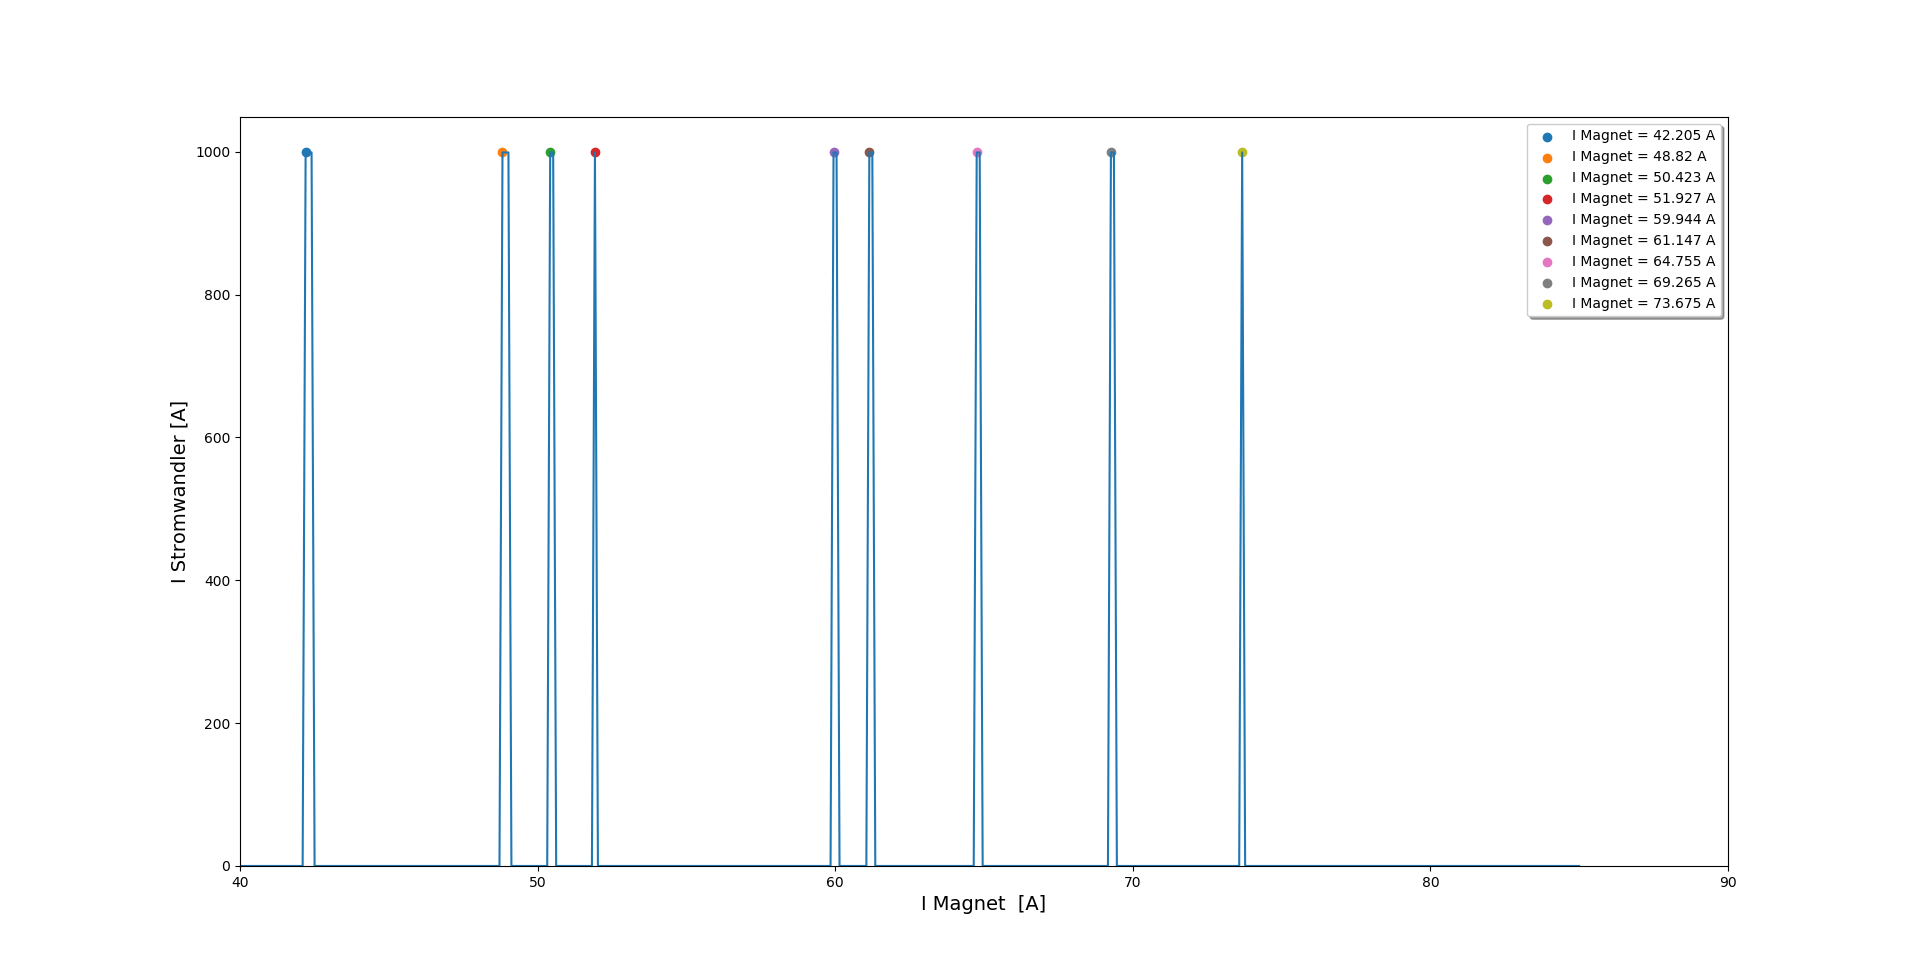
\includegraphics[width=.8\linewidth]{Pictures/LEMass40-85pos173KY13STUDPract.png}
\caption{Probe KY13}
\end{subfigure}%
\begin{subfigure}{.5\textwidth}
\centering
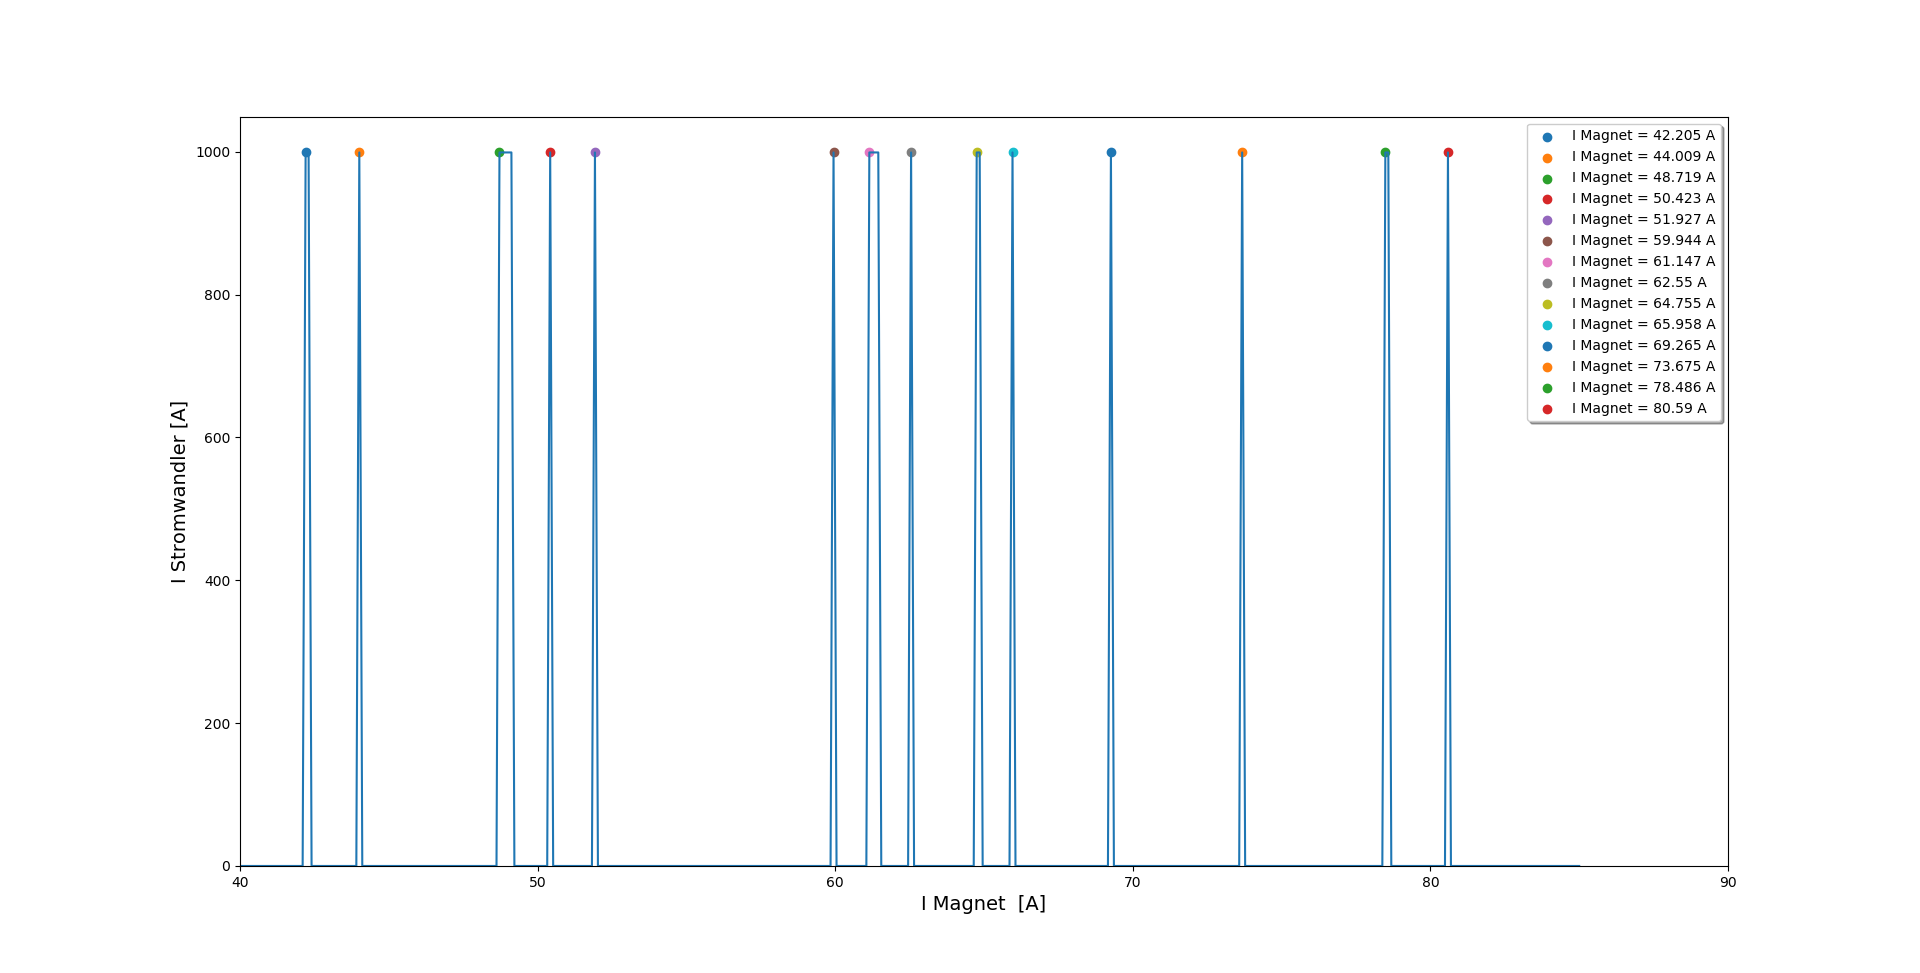
\includegraphics[width=.8\linewidth]{Pictures/LEMass40-85pos174KY14TUDPract.png}
\caption{Probe KY14}
\end{subfigure}%
\vskip\baselineskip
\begin{subfigure}{.5\textwidth}
\centering
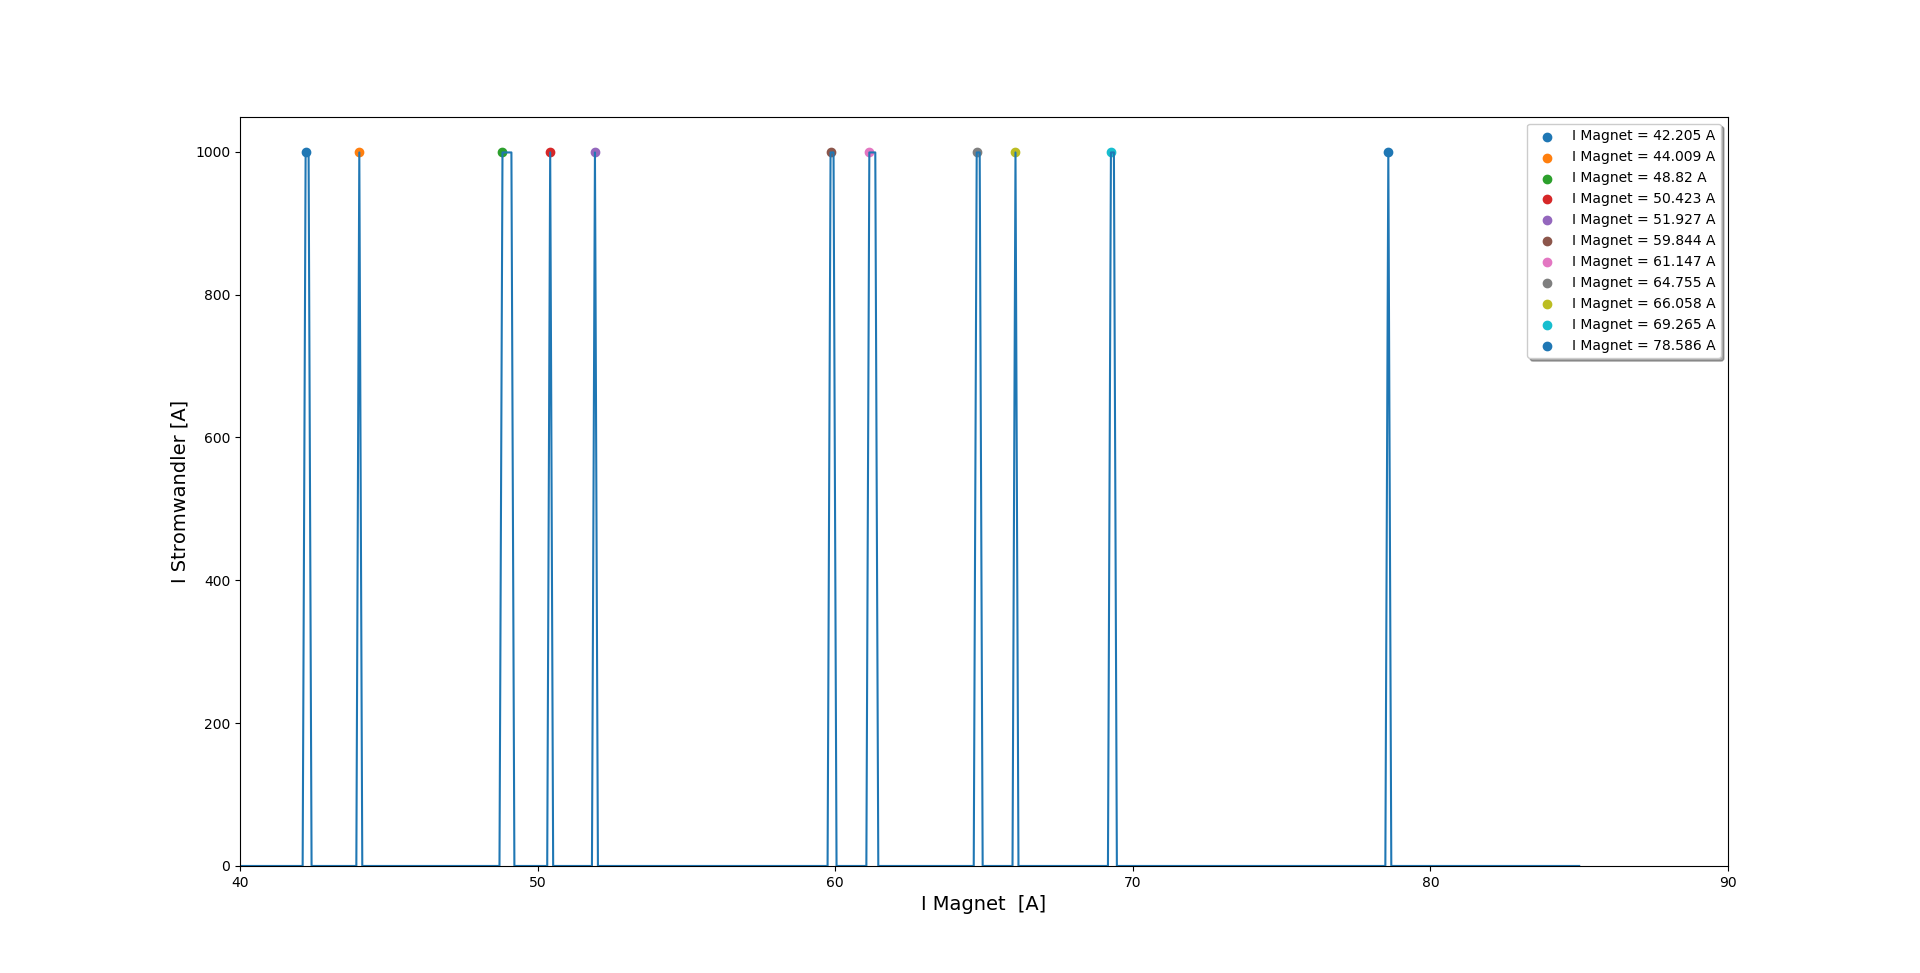
\includegraphics[width=.8\linewidth]{Pictures/LEMass40-85pos175KY16TUDPract.png}
\caption{Probe KY16}
\end{subfigure}%
\begin{subfigure}{.5\textwidth}
\centering
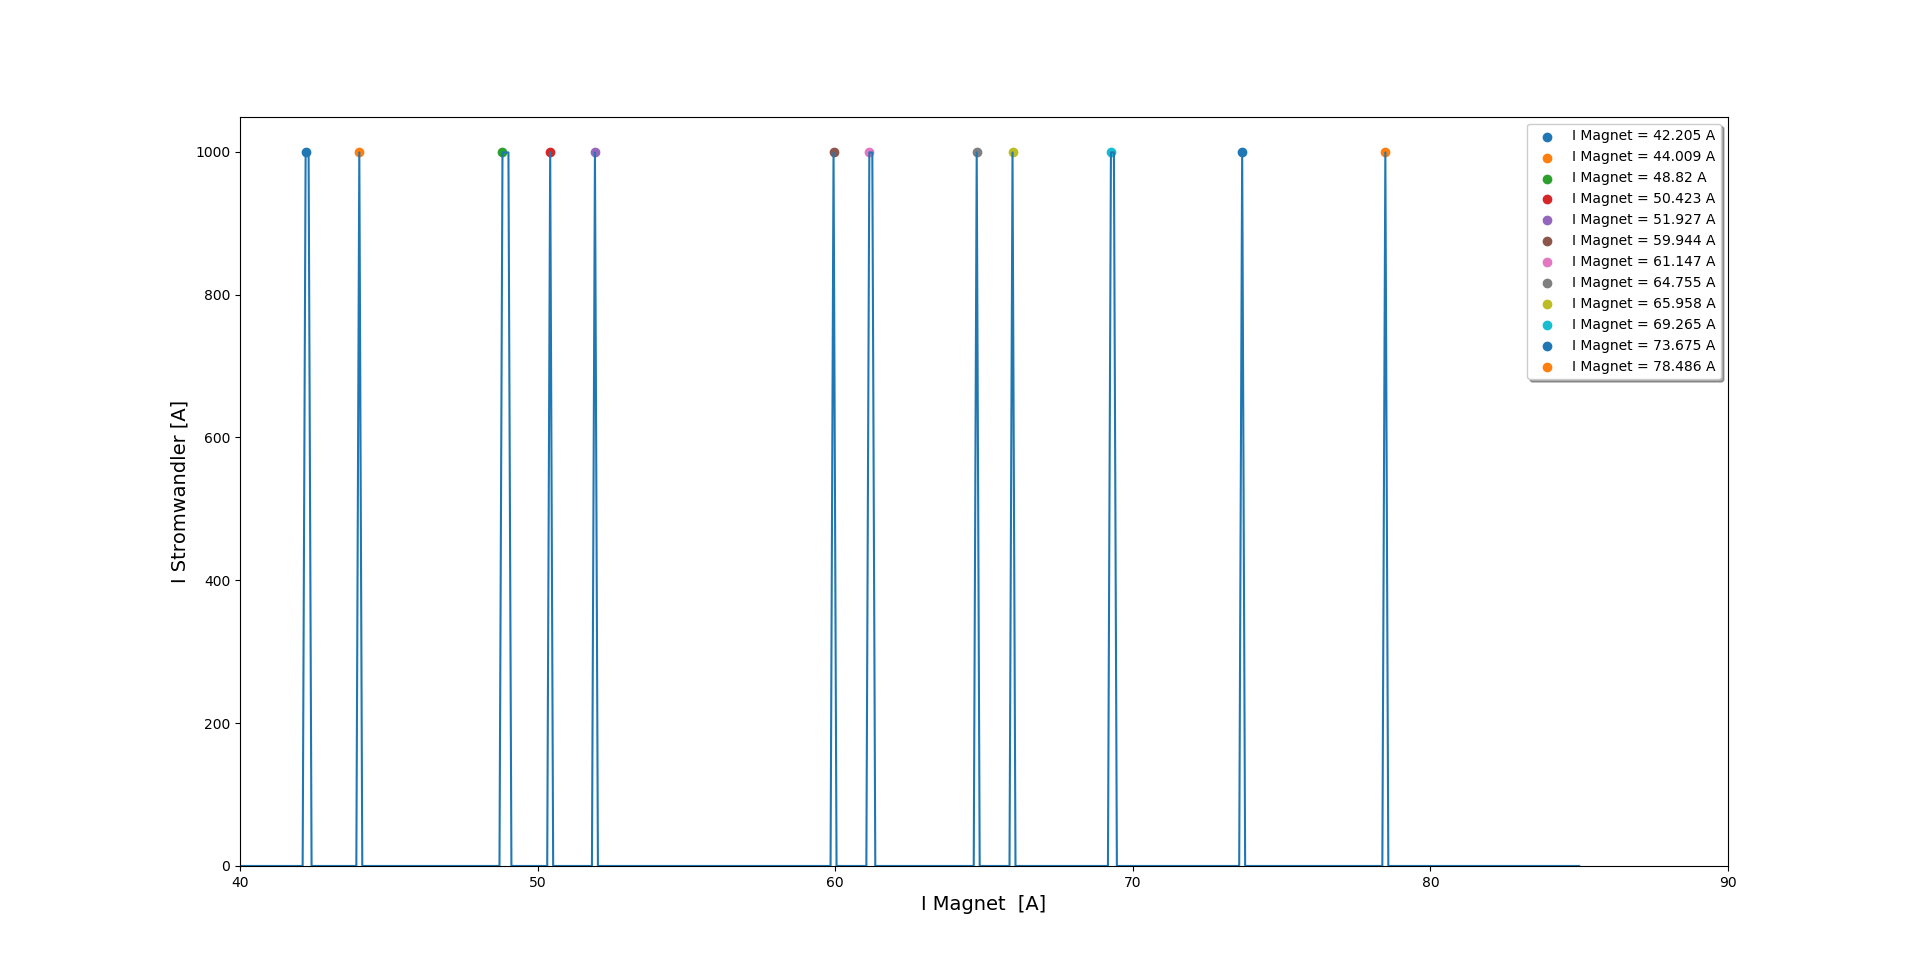
\includegraphics[width=.8\linewidth]{Pictures/LEMass40-85pos176KY17TUDPract.png}
\caption{Probe KY17}
\end{subfigure}%
\vskip\baselineskip
\begin{subfigure}{.5\textwidth}
\centering
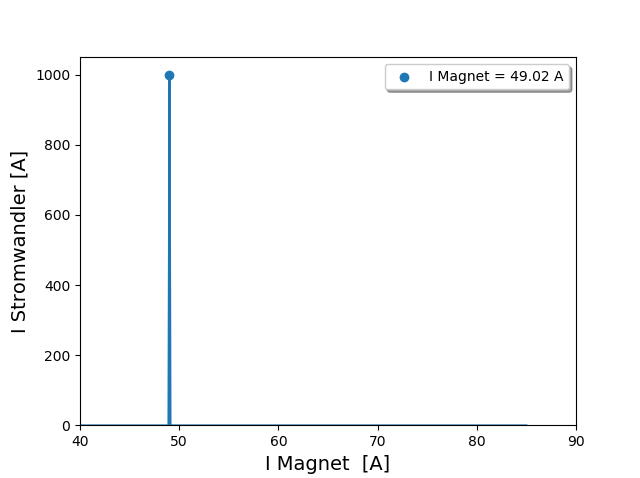
\includegraphics[width=.8\linewidth]{Pictures/153Be.png}
\caption{Probe 153BeO}
\end{subfigure}%
\caption{Gemessene Stromstärken für Strahlen in Abhängigkeit der eingestellten Stromstärke am Bi $90^{\circ}$ Bouncer Magneten für verschiedene Proben.}
\label{lowenergy}
\end{figure}

\clearpage

\subsection{Teilchenenergien nach dem Beschleuniger}
Die Vorselektierten Ionen werden im ersten Teil des Beschleunigers mit der angelegten Spannung beschleunigt.
In der Mitte treffen sie auf Argon an welchem sie sich umladen und die Moleküle aufbrechen.
(Das Aufbrechen der Moleküle ist kein Problem, da chemische Bindungsenergien typischerweise im \si{\electronvolt}-Bereich liegen, die Ionen bis dahin aber schon mehrere \si{\mega\electronvolt} an kinetischer Energie haben.)
Die entstandenen Ionen werden dann mit ihrer positiven Ladung noch ein weiteres Mal mit der angelegten Spannung beschleunigt.
Daher ergibt sich ihre Energie nach dem Beschleuniger zu:
\begin{gather}
    E_{\text{tot}} = e \cdot (U_{\text{Ionenquelle}} + U_{\text{Beschleuniger}}) \cdot \frac{m_{\text{Ion}^{+}}}{m_{\text{Molekül}^{-}}} + U_{\text{Beschleuniger}} \cdot q_{\text{Ion}^{+}}
\end{gather}
Wobei im erste Summand der Term $\frac{m_{\text{Ion}^{+}}}{m_{\text{Molekül}^{-}}}$ benutzt wird um die anteilige kinetische Energie des entstandenen Ions bis zum Argongas zu beschreiben.
Der zweite Summand beschreibt die Beschleunigung nach dem Argongas.

In unserem Versuch betrug die Spannung des Beschleunigers \SI{5.2479e6}{\volt}.
Damit ergeben sich für entstandene Ionen eine Energie nach dem Beschleuniger von:
\begin{center}
  \begin{tabular}{|c|c|}
    \hline
    Ion & Energie \\
    \hline
    $^{9}\text{Be}^{1+}$ & \SI{7.1}{\mega\electronvolt} \\
    $^{9}\text{Be}^{2+}$ & \SI{12.3}{\mega\electronvolt} \\
    $^{9}\text{Be}^{3+}$ & \SI{17.6}{\mega\electronvolt} \\
    $^{9}\text{Be}^{4+}$ & \SI{22.8}{\mega\electronvolt} \\
    \hline
    $^{10}\text{Be}^{1+}$ & \SI{7.3}{\mega\electronvolt} \\
    $^{10}\text{Be}^{2+}$ & \SI{12.5}{\mega\electronvolt} \\
    $^{10}\text{Be}^{3+}$ & \SI{17.8}{\mega\electronvolt} \\
    $^{10}\text{Be}^{4+}$ & \SI{23.0}{\mega\electronvolt} \\
    \hline
    $^{16}\text{O}^{1+}$ & \SI{8.5}{\mega\electronvolt} \\
    $^{16}\text{O}^{2+}$ & \SI{13.7}{\mega\electronvolt} \\
    $^{16}\text{O}^{3+}$ & \SI{19.0}{\mega\electronvolt} \\
    $^{16}\text{O}^{4+}$ & \SI{24.2}{\mega\electronvolt} \\
    \hline
  \end{tabular}
  \captionof{table}{Ionenenergien nach dem Beschleuniger für ausgewählte Ionen}
  \label{Auswertung_tab_Ionenenergien_nach_Besch}
\end{center}

\subsection{Faraday-Cups}
Nachdem wir nun Ionen mit hoher Geschwindigkeit nach dem Beschleuniger haben können wir versuchen häufig auftretende Nuklide nachzuweisen.
Aufgrund der hohen Anteile dieser Nuklide im Telichenstrahl entsteht durch sie ein nennenswerter Ladungsstrom der mit sogenannten Faraday-Cups gemessen werden kann.
Um einzelne Ionsorten detektieren zu können ist nach dem Beschleuniger ein \ang{90} Ablenkmagnet angebracht, der funktioniert wie der auf der Niederenergieseite.
Im Faraday-Cup werden dann die auftreffenden Ströme gemessen, die bei einem bestimmten Strom durch die Spule durch die abgelenkten Ionen entsteht.
Zunächst wollen wir sehen ob sich die Nuklide unserer BeO-Probe nachweisen lassen.
Dafür wurde in Abb. \ref{Auswertung_Bild_Faraday_Cup_BeO_HE} die gemessenen Ionenströme über dem Strom durch den Ablenkmagneten aufgetragen.
\begin{figure}[ht]
	\centering
           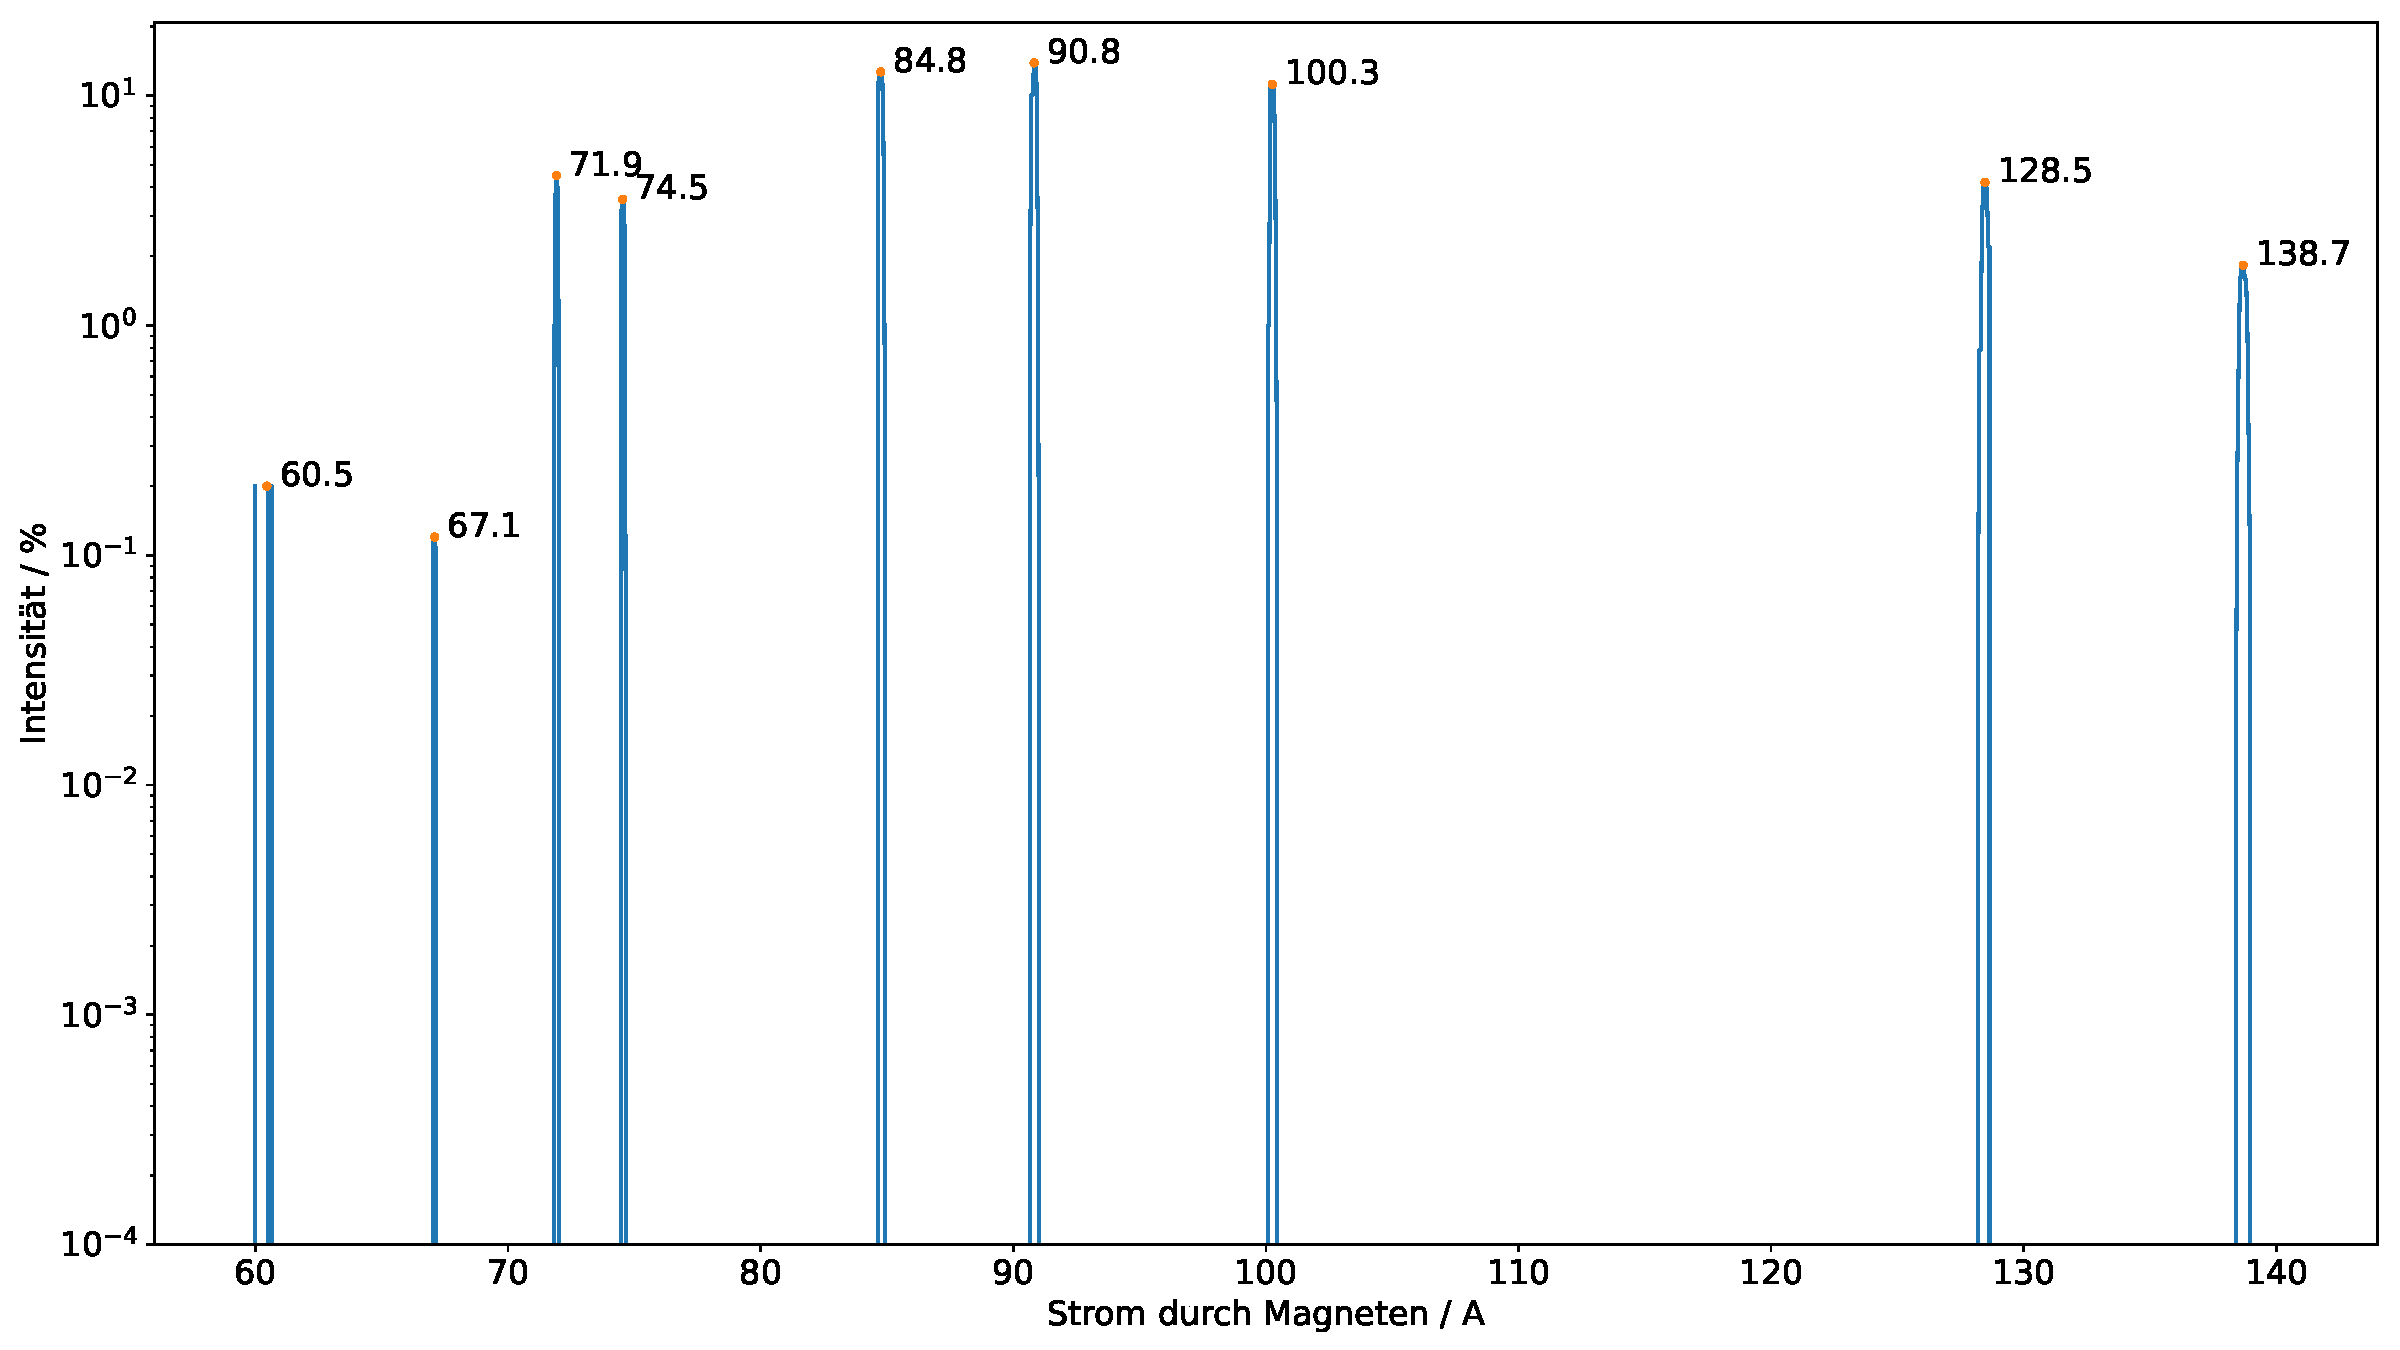
\includegraphics[width=0.85\textwidth]{Pictures/Faraday_Cup_BeO_HE.pdf}
	\caption{Strom gemessen im Faraday-Cup bei variieren des Magnetfeldes auf der Hochenergieseite für BeO-Probe. Die gemittelten x-Werte der Peaks sind eingezeichnet. Die Peaks wurden durch Vergleich mit umliegenden Werten gefunden. Die genaue Position wurde dann ermittelt indem die umliegenden Werte mit ihren Intensitäten als Wichtung gemittelt wurden.}
	\label{Auswertung_Bild_Faraday_Cup_BeO_HE}
\end{figure}

Da durch Massenfilterung nur Teilchen mit der gewählten Masse zu diesem Punkt kommen sollten, wurde für die BeO-Probe folgende Ionen als möglich erachtet:
\begin{center}
  \begin{tabular}{|c|c|c|c|}
    \hline
    Element & Masse $/\ \si{\atomicmassunit}$ & Ladungszustand $/\ e$ & $\frac{\sqrt{m_{\text{ion}}}}{q_{\text{ion}}}$\\
    \hline
    \multirow{8}*{Be}    & \multirow{4}*{$9$}  & $1+$                & \num{3}             \\
                         &                     & $2+$                & \num{1.5}           \\
                         &                     & $3+$                & \num{1}             \\
                         &                     & $4+$                & \num{0.75}          \\
    \cline{2-4}
                         & \multirow{4}*{$10$} & $1+$                & \num{3.16}          \\
                         &                     & $2+$                & \num{1.58}          \\
                         &                     & $3+$                & \num{1.05}          \\
                         &                     & $4+$                & \num{0.79}          \\
    \hline
    \multirow{4}*{O}     & \multirow{4}*{$16$} & $1+$                & \num{4}             \\
                         &                     & $2+$                & \num{2}             \\
                         &                     & $3+$                & \num{1.33}          \\
                         &                     & $4+$                & \num{1}             \\
    \hline
    \multirow{4}*{Al}    & \multirow{4}*{$26$} & $1+$                & \num{5.10}          \\
                         &                     & $2+$                & \num{2.55}          \\
                         &                     & $3+$                & \num{1.70}          \\
                         &                     & $4+$                & \num{1.27}          \\
    \hline
  \end{tabular}
  \captionof{table}{Mögliche Ionen auf Hochenergieseite für BeO-Probe.}
  \label{Auswertung_tab_moegl_ionen}
\end{center}

Mit Formel \ref{Auswertung_eq_Magnet} können wir jetzt wieder über die Verhältnisse der Magnetfelder auf die Ionenmassen schließen.
Dafür ist jedoch zuerst eine Kalibrierung des Magneten erforderlich. 
Um diese durchzuführen wurden verschiedene Stromstärken im erwarteten Arbeitsbereich eingestellt und die entsprechende magnetische Feldstärke gemessen.
Mit den so gewonnen Punkten wurde ein linearer Fit durchgeführt, der uns die Kalibriergerade gab.
Die Messdaten und Kurve sind in Abb. \ref{Magnet_kali} zu sehen, die Gerade ergab sich zu:
\begin{equation}
B(I) = ( [6,9 \pm 1,3] + [5,498 \pm 0,012] \cdot I ) \; mT.
\label{kali}
\end{equation}

\begin{figure}[ht]
  \centering
  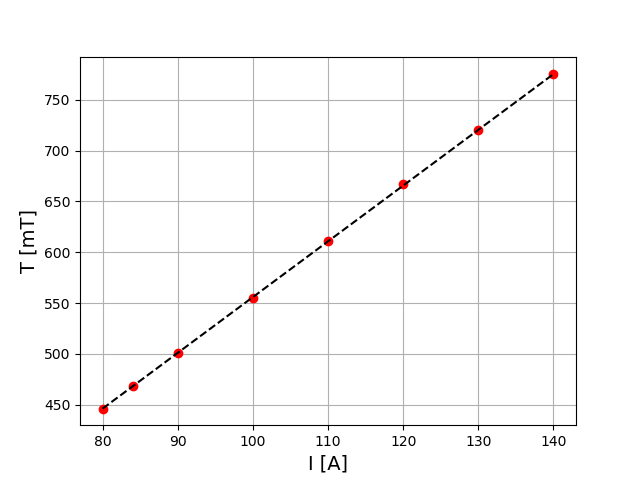
\includegraphics[width=0.7\linewidth]{Pictures/magnet.png}
  \caption{Kalibriergerade des Dipolmagneten.}
  \label{kali}
\end{figure}

Mit Kenntnis des Magneten, sowie der Energie, Masse und Ladung der Teilchen ist es uns jetzt möglich die erwartete Stromstärke für alle Ionen zu berechnen.
Diese folgt aus den Formeln \ref{Auswertung_eq_Magnet} und \ref{kali} zu;
\begin{equation}
I(E, m, q) = \frac{\frac{{\sqrt{2mE}}}{qr}-6,9}{5,498}
\label{HE_ion}
\end{equation}
Als Unsicherheit betrachten wir bei dieser Rechnung nur die Unsicherheit der Fitparameter.
Unsicherheiten durch Hysterese an den Magneten sollte zwar einen EInfluss haben, wird aber hier nicht beachtet.

Durch Kentniss des Magneten ist es uns jetzt möglich den Messpunkt eines bekannten Ions, in diesem Fall $^{10}$Be$^{2+}$, welches im Faraday-Cup gemessen wird.
Völlig analog zur Niedrigenergieseite ergibt sich das Magnetfeld hier zu $B \rho = \frac{p}{q} = \frac{\sqrt{wmE}}{q}$, mit dem Radius des Magneten $\rho = 1,5$ m.
Für $^{10}$Be$^{2+}$ ergibt sich damit mit der Energie nach Beschleunigung von $E = 12,5$ MeV: $B = 537$ mT.
Mit Formel \ref{kali} ergibt sich damit für die Stromstärke für $^{10}$Be$^{2+}$: $I = 96,4$ A, was uns wieder als Ausgangspunkt zur Identifikation des Strahls dient.
Die Masse für gemessene Stromstärken ergibt sich jetzt zu:
\begin{equation}
m_2 = m_1 \cdot \left( \frac{B_2}{B_1} \right)^2 = 10 \: \text{u} \cdot \left( \frac{I}{96.40} \right)^{2} \: \text{A}}
\end{equation}
Die so berechneten Massen sind in Tab. \ref{highenergy} zu sehen.
Durch betrachten der möglichen Verhältnisse von Ladung und Masse sowie Vergleich mit $^{10}$Be$^{2+}$ konnten dann die Teilchen identifiziert werden.
Zu beachten ist hier einerseits, dass wir nach dem Tandem eine vielzahl von Ladungszuständen erwarten und dass wir von einem Ion mit zweifach negativer Ladung ausgehen.
Auch zu beachten ist, dass wir die Messgenauigkeiten (z. B. Hystereseeffekte beim Magneten) hier nicht kennen, weshalb hier eine gewisse Abweichung zu erwarten ist.

\begin{table}[h]
\centering
\caption{Berechnung der Massen im Hochenergiebereich für Probe 153Be.}
\begin{tabular}{|c |c| c|}
\hline
I[A] & m[u] & Ion \\
\hline
60,5   & 4,0   &  $^{12}$C$^{2+}$  \\
67,1   & 4,9   &  $^{10}$Be$^{4+}$ \\
71,9   & 5,6   &  $^{9}$Be$^{3+}$\\
74,5   & 6,0   &  $^{10}$Be$^{3+}$\\
84,8   & 7,4   &  $^{16}$O$^{4+}$ \\
90,8   & 8,9   &  $^{9}$Be$^{2+}$ \\
100,3 & 10,8 &  $^{26}$Al$^{4+}$\\
128,5 & 17,7 &  $^{16}$O$^{2+}$\\
138,7 & 20,7 &  $^{9}$Be$^{1+}$ \\
\hline
\end{tabular}
\label{highenergy}
\end{table}

Dabei ist zu beachten, dass $^{10}\text{B}$ nicht von $^{10}\text{Be}$ unterschieden werden kann und es daher auch keinen Sinn macht es mit aufzunehmen.
Isobare können erst im weiteren Verlauf getrennt werden.
Das Vorhandensein von $^{26}$Al$^{4+}$ lässt sich ebenfalls damit erklären, dass dieses Aufgrund seiner Masse bisher nicht magnetisch herausgefiltert wurde.
Wie bereits im Niedrigenergiebereich erwähnt, ist dieses schwer vom BeO zu trennen.
Nicht beachtet wurden hier die verschiedenen Sauerstoffisotope, da diese relativ selten selten sind.
Prinzipiel wäre es durch Kentnis des Magneten mit den Formeln \ref{Auswertung_eq_Magnet} und \ref{kali} auch möglich direkt die erwartete Stromstärke eines Ions zu berechnen und durch vergleich der erwarteten mit den berechneten auf die Ionen zu schließen.
Dabei wäre es jedoch nachteilig, dass ohne Verhältnisbildung die Unsicherheiten der Messung weniger eliminiert werden, welche uns nicht bekannt sind.

\clearpage

\subsection{Isobarentrennung}
Wie in dem vorherigen Abschnitt bereits erwähnt ist es bis hierhin noch nicht möglich gewesen Isobare zu unterscheiden.
Um Abhilfe zu schaffen ist im weiteren Strahlenverlauf eine dünne Schicht aus Siliziumnitrid angebracht.
Da der Verlust an kinetischer Energie von Atomen in Materie stark von der Kernladungszahl abhängt erlaubt dies die Isobarentrennung.
den Faktor $\frac{\Delta E}{\Delta x}$ erhalten wir aus der frei verfügbaren Software SRIM.
Für $^{10}\text{Be}$ ist $\left (\frac{\Delta E}{\Delta x}\right )_{^{10}\text{Be}} = \SI{766.7}{\kilo\electronvolt\per\micro\metre}$.
Die SiN-Folie hat eine Dicke von \SI{1}{\micro\metre}.
Damit ergibt sich ein Energieverlust der $^{10}\text{Be}$-Atome von \SI{766.7}{\kilo\electronvolt}.
Die verbleibende Energie der $^{10}\text{Be}$-Ionen ist dann, abhängig von deren Energie vorher:
\begin{center}
  \begin{tabular}{|c|c|c|}
    \hline
    Ion & Energie nach Beschleuniger & Energie nach Folie \\
    \hline
    $^{10}\text{Be}^{1+}$ & \SI{7.3}{\mega\electronvolt}  & \SI{6.5}{\mega\electronvolt}  \\
    $^{10}\text{Be}^{2+}$ & \SI{12.5}{\mega\electronvolt} & \SI{11.6}{\mega\electronvolt} \\
    $^{10}\text{Be}^{3+}$ & \SI{17.8}{\mega\electronvolt} & \SI{17.0}{\mega\electronvolt} \\
    $^{10}\text{Be}^{4+}$ & \SI{23.0}{\mega\electronvolt} & \SI{22.3}{\mega\electronvolt} \\
    \hline
  \end{tabular}
  \captionof{table}{Ionenenergien nach ser SiN Folie in Abhängigkeit der Ladungszustände aus dem Beschleuniger.}
  \label{Auswertung_tab_Ionenenergien_nach_Folie}
\end{center}
Nach der Folie wird $^{10}\text{Be}$ nur noch im Ladungszustand $4+$ erwartet, da die Atome durch die Foile weiter ionisiert werden.

Um nun die Isobare $^{10}\text{Be}$ und $^{10}\text{B}$ zu trennen ist nach der Folie ein elektrostatischer Analysierer angebracht.
Die Spannung die angelegt werden muss kann berechnet werden durch Kräftegleichgewicht:
\begin{gather}
    q_{\text{Ion+}} \cdot \frac{U_{\text{Platte}}}{d_{\text{Platte}}} = \frac{mv^{2}}{r}
\end{gather}
Wobei $d_{\text{Platte}} = \SI{3.6}{\centi\metre}$ und $r = \SI{2.6}{\metre}$ ist.
Die Spannung, die einzustellen ist, ist jedoch nur die halbe, da auf den Platten jeweils $+U_{\text{Platte}}$ und $-U_{\text{Platte}}$ erzeugt wird (die Spannung wird beim einstellen relativ zur Erdung gemessen).
Für das Ion $^{10}\text{Be}^{4+}$ ergibt sich daher in Abhängigkeit der Energie nach der Folie eine Ablenkspannung von:
\begin{center}
  \begin{tabular}{|c|c|c|}
    \hline
    Ion & Energie nach Folie & $\frac{U_{\text{Platte}}}{2}$ \\
    \hline
    \multirow{4}*{$^{10}\text{Be}^{4+}$} & \SI{6.5}{\mega\electronvolt}  & \SI{22.5}{\kilo\volt} \\
                                         & \SI{11.6}{\mega\electronvolt} & \SI{40.7}{\kilo\volt} \\
                                         & \SI{17.0}{\mega\electronvolt} & \SI{58.9}{\kilo\volt} \\
                                         & \SI{22.3}{\mega\electronvolt} & \SI{77.0}{\kilo\volt} \\
    \hline
  \end{tabular}
  \captionof{table}{Ablenkspannug für den ESA für verschiedene Ionenenergien.}
  \label{Auswertung_tab_Ablenkspannung_ESA}
\end{center}
